\documentclass[conference]{IEEEtran}
\IEEEoverridecommandlockouts
% The preceding line is only needed to identify funding in the first footnote. If that is unneeded, please comment it out.
\usepackage{cite}
\usepackage{amsmath,amssymb,amsfonts}
\usepackage{algorithmic}
\usepackage{graphicx}
\usepackage{textcomp}
\usepackage{xcolor}
\usepackage[english, brazil]{babel}
\def\BibTeX{{\rm B\kern-.05em{\sc i\kern-.025em b}\kern-.08em
    T\kern-.1667em\lower.7ex\hbox{E}\kern-.125emX}}
\begin{document}

\title{Análise da inflência da renda familiar na evasão de alunos no Insituto Federal de Educação, Ciência e Tecnologia de São Paulo}

\author{\IEEEauthorblockN{Luiz Roberto Albano Junior}
\IEEEauthorblockA{\textit{Faculdade de Energia Elétrica e de Computação} \\
\textit{Universidade Estadual de Campinas}\\
Campinas, Brasil \\
l272746@g.unicamp.br}
\and
\IEEEauthorblockN{Tárcio Augusto Canhamina Quissanga}
\IEEEauthorblockA{\textit{Faculdade de Energia Elétrica e de Computação} \\
\textit{Universidade Estadual de Campinas}\\
Campinas, Brasil \\
t214551@dac.unicamp.br}
}

\maketitle

\selectlanguage{brazil}
\begin{abstract}
Resumo do trabalho\\
\textbf{Palavras chave: } palavra1, palavra2
\vspace{2.5mm}
\end{abstract}

\selectlanguage{english}
\begin{abstract}
Abstract of article\\
\textbf{Keywords: } word1, word2
\end{abstract}

\section{Introdução}
Um dos maiores desafios enfrentados pelas instituições de ensino é o problema da evasão de estudantes. Este problema complexo que pode se originar de diversos fatores e que impacta diretamente tanto estudantes quanto o funcionamento das instituições educacionais \cite{oliveira2021}.\par
Podemos definir a evasão como a saída definitiva do estudante de seu curso de origem, sem concluí-lo. As formas de evasão podem ocorrer de diversas maneiras, como o abandono do estudantes às aulas, exauridas as tentativas de contato, pela desistência formalizada pelo estudante, a transferência para outra instituição ou a exclusão por ação institucional \cite{silveira2021}.\par
No contexto da Instituto Federal de Educação, Ciência e Tecnologia de São Paulo (IFSP), a evasão compromete o funcionamento e a eficiência da instituição, causando impacto financeiro significativo. Este impacto é causado pela perda de receitas, enquanto os custos operacionais permanecem inalterados, podendo resultar na ociosidade de professores, funcionários, equipamentos e espaços físicos, representando um desperdício de recursos públicos ou a depracação destes serviços \cite{silveira2021}.\par
Diversos fatores contribuem para a evasão escolar. De forma externa, analisando o lado do estudante, podemos destacar fatores como formação educacional deficitária, falta de identificação com o curso escolhido e problemas socioeconômicos, objetivo de análise deste artigo, como a baixa renda familiar ou a necessidade de conciliar trabalho e estudo. Além disso, problemas internos como disciplinaas com alto grau de dificuldades, falta de preparo pedagógico de docentes e a carga horária de alguns cursos agragavam a situação dos estudantes.\par
Compreender a evasão escolar no IFSP, e em outras instituições de ensino, exige uma atenção e esforços contínuos para identificação dos fatores e variáveis que contribuem com o problema, além de esforços coordenados para redução do problema, mantendo os alunos na instituição e possivelmente assegurando que eles tenham uma experiência educacional mais significativa e de qualidade.\par
O propósito deste trabalho é avaliar a partir de dados abertos disponíveis na plataforma Plataforma Nilo Peçanha (PNP) \cite{pnp2024}, 
se a evasão dos estudantes desta instituição são influênciadas pela renda familiar. Serão utilizadas ferramentas como gráficos e de conceitos de análise estatística, de hipóteses e estatísticas de teste que possam confirmar a afirmação inicial, ou hipótese nula ("H-nada") \cite{ismay2024}, de que a evasão dos alunos do Instituto Federal de São Paulo (IFSP) não é influenciada pela renda familiar. Além disto tentar identificar outras possíveis variáveis da base de dados poderiam causar influência na evasão escolar.\par


\section{Materiais e Métodos}
Para realização deste estudo utilizamos os microdados referêntes às matrículas dos estudantes, contidos no Portal de Dados Abertos do Ministério da Educação - Plataforma Nilo Peçanha (PNP) \cite{pnpdados2024}. A base de dados escolhida \cite{microdados2021} foi a mais recente disponível no momento do acesso, representando um conjunto de dados de matrículas de estudantes que estiveram pelo menos um dia do ano base de 2020.\par
A documentação foi realizada em um \textit{notebook Python} disponível em \cite{notebook}. Para elaboração do \textit{notebook} foi utilizada a linguagem Python \cite{python2024} e bibliotecas para manipulação, análise de dados, computação de modelos estatísticos e análise visual de dados, sendo: Pandas \cite{pandas2024}, NumPy \cite{numpy2024}, Plotnine \cite{plotnine2024}, Matplotlib \cite{matplot2024}, Seaborn \cite{seaborn2024}, SciPy \cite{scipy2024} e Statsmodel \cite{statsmodel2024}.\par
O primeiro passo foi realizar uma visualização bruta de alguns dados para visualização de categorias de valores e realização da limpeza de dados inexistentes que pudessem comprometer as futuras análise e exploração das variáveis. O passo seguinte foi a exploração e análise dos dados, através de histogramas para podermos visualizar e entender o comportamento das principais variáveis presentes na base de dados escolhida. Como a base de dados contém informações de matrículas de toda rede federal de ensino, realizamos um filtro na coluna "Instituição" para o valor "IFSP", a fim de aproximar do objetivo de nossa análise.\par

\begin{figure}[h]
    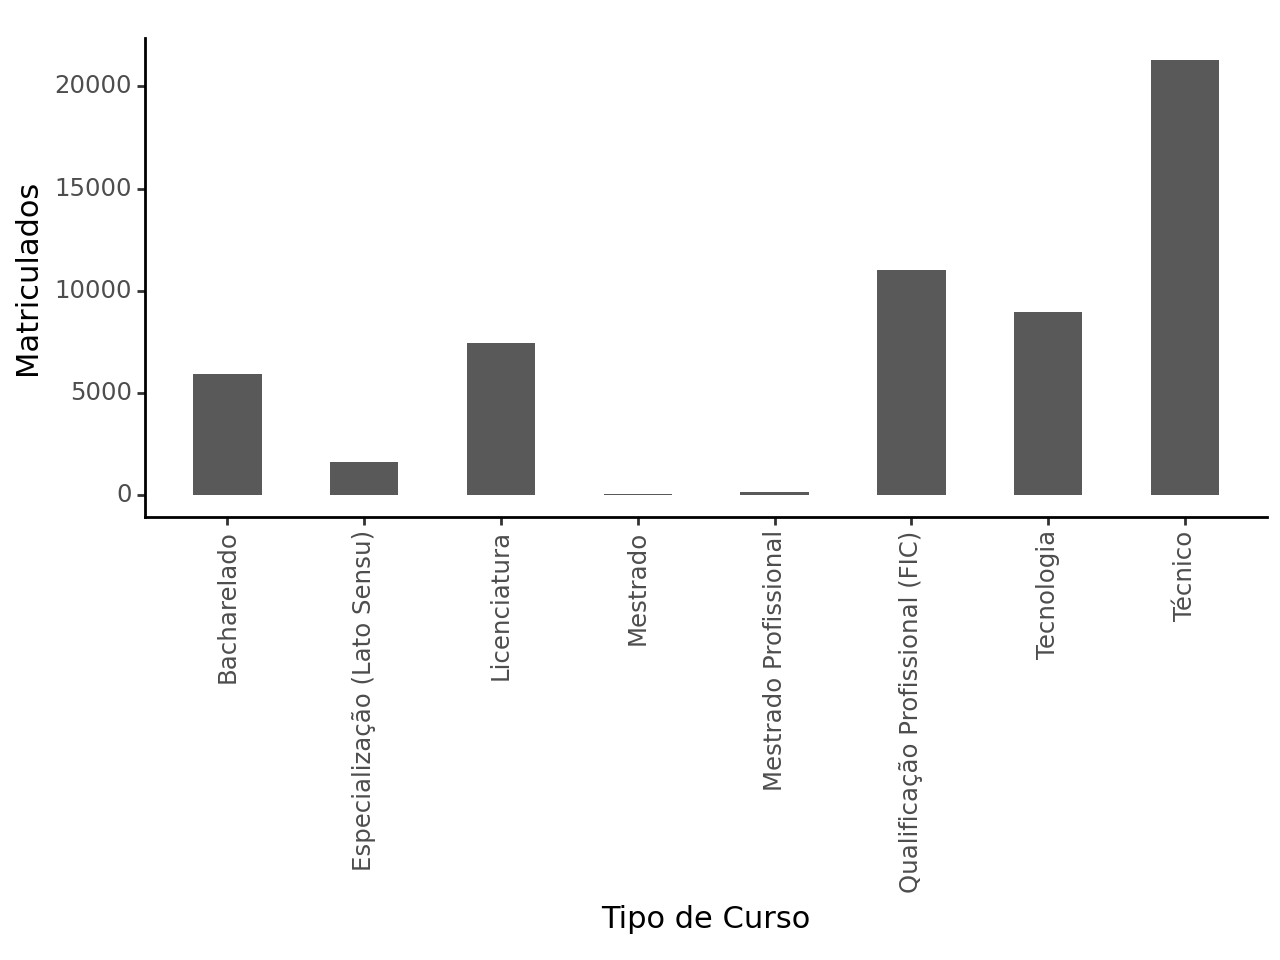
\includegraphics[width=8.9cm]{figs/histograma-tipos-cursos.png}
    \centering
\end{figure}

Esta análise inicial pôde determinar a necessidade de filtros adicionais


\section{Resultados}
Texto da seção

\section{Discussão}
Texto da seção

\section{Conclusões}
Texto da seção

\section*{Referências Bibliográficas}

\begin{thebibliography}{00}

\bibitem{ismay2024}ISMAY, C.; KIM, A. Y. Statistical Inference via Data Science - A ModernDive into R and the Tidyverse. Disponível em: https://moderndive.com. Acesso em: 14 jun. 2024.

\bibitem{plotnine20204}KIBIRIGE, H. plotnine 0.13.6 - A Grammar of Graphics for Python. Disponível em: https://plotnine.org. Acesso em: 26 jun. 2024.

\bibitem{microdados2021}MINISTÉRIO DA EDUCAÇÃO. 2020 - Microdados Matrículas - Portal de Dados Abertos do Ministério da Educação. Disponível em: https://dadosabertos.mec.gov.br/pnp/item/134-2020-microdados-matriculas. Acesso em: 14 jun. 2024. 

\bibitem{pnpdados2024} MINISTÉRIO DA EDUCAÇÃO. PNP - Dados Abertos - MEC. Disponível em: https://dadosabertos.mec.gov.br/pnp. Acesso em: 14 jun. 2024.

\bibitem{pnp2024} MINISTÉRIO DA EDUCAÇÃO. PNP - Plataforma Nilo Peçanha. Disponível em: https://www.gov.br/mec/pt-br/pnp. Acesso em: 13 jun. 2024.

\bibitem{pandas2024} NUMFOCUS, INC. pandas - Python Data Analysis Library. Disponível em: https://pandas.pydata.org/. Acesso em: 26 jun. 2024.

\bibitem{numpy2024}NUMPY TEAM. NumPy. Disponível em: https://numpy.org. Acesso em: 26 jun. 2024.

\bibitem{oliveira2021} OLIVEIRA, Francisco Lidoval de; NÓBREGA, Luciano. Evasão escolar: um problema que se perpetua na educação brasileira. Revista Educação Pública, v. 21, nº 19, 25 de maio de 2021. Disponível em: https://educacaopublica.cecierj.edu.br/artigos/21/19/evasao-escolar-um-problema-que-se-perpetua-na-educacao-brasileira. Acesso em 25/06/2024.

\bibitem{statsmodel2024}PERKTOLD, J.; SEABOLD; TAYLOR, J. Statsmodels - statistical models, hypothesis tests, and data exploration. Disponível em: https://www.statsmodels.org/stable/index.html. Acesso em: 26 jun. 2024. 

\bibitem{python2024} PYTHON SOFTWARE FOUNDATION. Welcome to Python.org. Disponível em: https://www.python.org. Acesso em: 26 jun. 2024. 

\bibitem{scipy2024}SCIPY. SciPy. Disponível em: https://scipy.org. Acesso em: 26 jun. 2024. 

\bibitem{silveira2021} SILVEIRA, Fernanda Romanezi da
A evasão de estudantes no IFSP: uma contribuição ao
conhecimento das dificuldades na identificação de seus
determinantes / Fernanda Romanezi da Silveira. – São Paulo :
EDIFSP, 2021. 306 p. – (Selo Teses \& Dissertações)

\bibitem{matplot2024}THE MATPLOTLIB DEVELOPMENT TEAM. Matplotlib: Visualization with Python. Disponível em: https://matplotlib.org. Acesso em: 26 jun. 2024. 

\bibitem{seaborn2024}WASKOM, M. Seaborn: statistical data visualization. Disponível em: https://seaborn.pydata.org. Acesso em: 26 jun. 2024.

\end{thebibliography}

\end{document}
